\chapter{Results}
\label{chapter:results}
In this chapter we will discuss the results of our experiments with groups. Note that the \textbf{error rate} depicted in the graphs is \textit{not} the loss, but rather its square root. This is done in order to represent errors on the original scale.

\section{Cyclic groups}
Cyclic groups are the simplest groups possible. They are defined as groups generated by only one element $x$. They are all isomorphic to either $(\mathbb{Z},+,-,0)$ - integers with addition - or $(\mathbb{Z}_n,+,-,0)$ : $\{0,1,2,\dots n-1\}$ with addition modulo $n$. They are all commutative.

\subsection{Example network for addition in $\mathbb{Z}_n$}
\label{section:addition example}
Here we will show an example of how a network that computes $Z_n$ may look like. One such network for $n=2$ is illustrated in \Autoref{section:xor}, since Xor on $\{0,1\}$ is identical to addition modulo 2. For other $n\in \mathbb{N}$, we will use a different network.

This network will have two layers, therefore it has the form $$f(\textbf{x})=\textbf{w}^\top \alpha\left(\textbf{W}_2(\alpha(\textbf{W}_1\textbf{x}+\textbf{c}_1))+\textbf{c}_2\right)$$ where $\textbf{W}_1,\textbf{W}_2$ are weight matrices, $\textbf{c}_1,\textbf{c}_2$ are bias vectors and $\alpha$ is an activation function.

We will set 
$$\textbf{W}_1=
	\left(\begin{matrix}
		1 & 1\\
		1 & 1
	\end{matrix}\right), 
\textbf{W}_2=
	\left(\begin{matrix}
		1 & -2n\\
		0 & 1
	\end{matrix}\right)$$
	and
$$\textbf{c}_1=
	\left(\begin{matrix}
		0\\
		-n+1
	\end{matrix}\right),
\textbf{c}_2=
	\left(\begin{matrix}
		0\\
		-1
	\end{matrix}\right),
\textbf{w}=
	\left(\begin{matrix}
		1 \\
		1
	\end{matrix}\right)$$
We set $\alpha$ to be the ReLU function, just like in the XOR example.

This network exactly computes $a+b$ (mod 10), where $\textbf{x}=(a,b)^\top$ and $0\leq a,b<n$.

The first layer is $\alpha(\textbf{W}_1\textbf{x}+\textbf{c}_1)$. That is 
$$\alpha\left(
\left(\begin{matrix}
		1 & 1\\
		1 & 1
	\end{matrix}\right)
\left(\begin{matrix}
	a\\
	b
\end{matrix}\right)
+
\left(\begin{matrix}
	0\\
	-n+1
\end{matrix}\right)
\right)
=
\alpha\left(
\left(\begin{matrix}
	a+b\\
	a+b
\end{matrix}\right)
+
\left(\begin{matrix}
	0\\
	-n+1
\end{matrix}\right)
\right)
=$$
$$=
\alpha\left(
\left(\begin{matrix}
	a+b\\
	a+b-n+1
\end{matrix}\right)
\right)
$$

We will call the output of the first layer $(y_1,y_2)^\top$. We have two possibilities for $a+b$. Either $a+b\geq n$, then both $y_1,y_2> 0$, or $a+b< n$, then $a+b-n+1\leq 0$, so $y_2=0$. We see that after the application of $\alpha$, at most one of the elements $y_1,y_2$ is non-zero. 

Next we apply the second layer: 
$$\alpha\left(
\left(\begin{matrix}
		1 & -2n\\
		0 & 1
	\end{matrix}\right)
\left(\begin{matrix}
	y_1\\
	y_2
\end{matrix}\right)
+
\left(\begin{matrix}
	0\\
	-1
\end{matrix}\right)
\right)
=
\alpha\left(
\left(\begin{matrix}
	y_1-2ny_2\\
	y_2
\end{matrix}\right)
+
\left(\begin{matrix}
	0\\
	-1
\end{matrix}\right)
\right)
=$$
$$=
\alpha\left(
\left(\begin{matrix}
	y_1-2ny_2\\
	y_2-1
\end{matrix}\right)
\right)
$$

We will call output of this layer $(z_1,z_2)^\top$. 

If we have $a+b\geq n$, therefore $y_1=a+b, y_2=a+b-n+1$, we have $y_1-2ny_2<0$ (because $y_2\geq 1$ and $a+b<2n$), therefore $z_1=0$. In this case also $z_2=a+b-n=(a+b)\text{mod}\ n$.

If we have $a+b< n$, therefore $y_1=a+b,y_2=0$, we have $z_1=a+b=(a+b)\text{mod}\ n$, $z_2=0$ (because $y_2-1<0$).

We see that one of $z_1,z_2$ always has the desired result, while the other is zero. Therefore the output layer $\textbf{w}^\top \left(\begin{matrix}
z_1\\
z_2
\end{matrix}\right)=z_1+z_2$ always gives the correct value.

Since we did not assume that $a,b$ are natural numbers, this network is also stable under commutative algebraic extensions of $\mathbb{Z}_n$, i.e. it does not need any modification to work correctly with fractions (or even irrationals).
\subsection{$\mathbb{Z}_{10}$}

\begin{itemize}
	\item[\textbf{Elements:}] Integers $0,1,2,\dots,9$
	\item[\textbf{Operations:}] Composition is addition modulo 10, inverse of $a$ is $10-a$ and the unit is 0.
	\item[\textbf{Grounding:}] As themselves in $\mathbb{R}^1$
	\item[\textbf{Extension:}] Using the equation $h+h=1$. Because $h+h$ is "even", we can see that the base group has no solution. We call this $h$ "half".
	\item[\textbf{Notes:}] Since $\mathbb{Z}_{10}$ is commutative, we want the extension to be commutative as well (see Theorem\autoref{theorem:abelian uniqueness}). We expect to get an extension isomporphic to $\mathbb{Z}_{20}$.
\end{itemize}

The learning progress of one experiment with training the composition, inverse and the unit is depicted in \Autoref{graph:z10_90percent}. The (logarithmic) error rate on the Y axis is the square root of loss (to closer resemble Euclidean distance).

The curve depicting the error rate of the inverse appears smoother. That is because the testing set for the inverse network contains 10\% of all data, therefore here it is only one element. That means that all testing batches are the same (although that is not true for thes training batches).

One unexpected result was the fact that while in most runs the unit tended to be around $0$, sometimes it also settled around $10$. That could also be considered a right answer, although $10$ is not in the chosen representation.\\

While learning the extension, most of the time the "half" settled around $5.5$. This is of course one of two possible intuitive solutions to $a+a=1(\text{mod} 10)$, the other of course being $0.5$. Table \ref{table:z10_half} shows how the extension settled in several different runs. Note that the runs had different lengths, but the \textit{half} always settled so early that the length had no effect.

Table \ref{table:z10_half_generator} shows how two different runs generated the extension (isomorphic to $\mathbb{Z}_{20}$) using iterated (learned) composition on the "half" element.

\begin{figure}[b]
\caption{Error rate for the learning of composition, inverse and unit in $\mathbb{Z}_{10}$ on the testing data. Testing data percentage is 10\%. Each epoch describes one optimization step.}
\label{graph:z10_90percent}
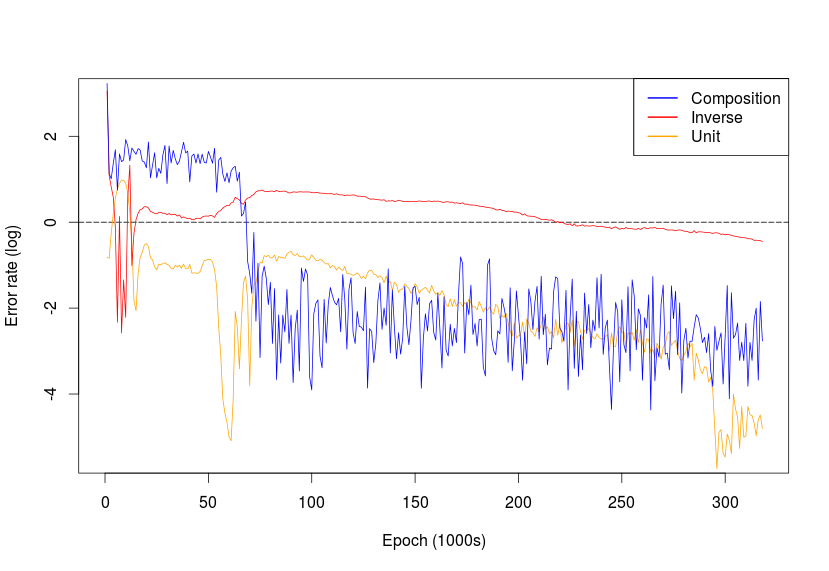
\includegraphics[width=\linewidth]{../img/z10_90percent.png}
\end{figure}
\begin{figure}[h]
\centering
\caption{Different values of "half" found during different runs. The first run (red) was very peculiar since it had over 2 700 000 epochs, but this representation settled already around epoch 300 000. It is not clear how this interacts with the rest of the elements.}
\label{table:z10_half}
\begin{tabular}{|c|c|c|c|c|c|}
\hline
\textcolor{red}{-0.9417969} & \textcolor{blue}{5.5017343} & \textcolor{blue}{5.500125} & 0.5014977 & \textcolor{blue}{5.500004} & \textcolor{blue}{5.507943}\\
\hline
\end{tabular}
\end{figure}

\begin{figure}[h]
\centering
\caption{Extension groups generated in two runs (read left to right, top to bottom). The blue elements are supposed to be in the original embedding, i.e. they should be 1...9 ascending with the last 3 elements being 0, "half", 1 respectively. In the first run we see that we have had very low success, even though the first half+half looks promising. The second run had much better success and with the exception of 9 it hit all original elements reasonably well, even those last 3.}
\label{table:z10_half_generator}
\begin{tabular}{ccccc}
\textbf{5.500004} & \textcolor{blue}{0.99998194} & 10.919293 & \textcolor{blue}{6.419118} & 1.9191066\\
 \textcolor{blue}{9.268123} & 4.7680063 & \textcolor{blue}{0.26805452} & 12.234171 & \textcolor{blue}{7.7339497}\\
3.2338893 & \textcolor{blue}{8.733828} & 4.233731 & \textcolor{blue}{1.9053116} & 9.292908 \\
\textcolor{blue}{4.792793} & 0.2928396 & \textcolor{blue}{12.189646} & 7.6894255 & \textcolor{blue}{3.1893663}\\
\textbf{8.689303} & \textcolor{blue}{4.189211}\\
 \\
\hline\\

\textbf{5.5069175} & \textcolor{blue}{0.99456155} & 6.5232387 & \textcolor{blue}{2.0135} & 7.5396843\\
\textcolor{blue}{3.032562} & 8.556266 & \textcolor{blue}{4.051762} & 3.872835 & \textcolor{blue}{5.4972463}\\
0.9848655 & \textcolor{blue}{6.5135655} & 2.0038028 & \textcolor{blue}{7.530016} & 3.022867\\
\textcolor{blue}{8.546589} & 4.04206 & \textcolor{blue}{3.9609222} & 4.6975384 & \textcolor{blue}{0.18309715}\\
\textbf{5.713754} & \textcolor{blue}{1.20193}
\end{tabular}

\end{figure}


\subsection{$\mathbb{Z}_{20}$}
The second group we experimented with was $\mathbb{Z}_{20}$. Because of its larger size, the experiments with it were longer. 

\begin{itemize}
	\item[\textbf{Elements:}] Integers $0,1,2,\dots,19$
	\item[\textbf{Operations:}] Composition is addition modulo 20, inverse of $a$ is $20-a$ and the unit is 0.
	\item[\textbf{Grounding:}] As themselves in $\mathbb{R}^1$
	\item[\textbf{Extension:}] Using the equation $h+h=1$. As with $\mathbb{Z}_{10}$, this has no solution in $\mathbb{Z}_{20}$.
	\item[\textbf{Notes:}] Once again we expect a commutative extension, this time isomporphic to $\mathbb{Z}_{40}$.
\end{itemize}

The error rates during one experiment can be seen in \Autoref{graph:z20_90percent}. Once again, $10\%$ was excluded from the training. The trend lines are similar to $\mathbb{Z}_{10}$ (\Autoref{graph:z10_90percent}), with composition and inverse training quickly, while inverse lags behind. The inverse line is much noisier than with $\mathbb{Z}_{10}$, because now the testing data has 2 elements, out of which 5 are chosen for testing (with repetition).

Values for the half in different runs can be seen in \Autoref{table:z20_half}. Once again, the algorithm usually found one of the two intuitive answers, 0.5 and 10.5. A graph showing the iterated composition of the half is depicted in \Autoref{graph:z20_half_generator}. As we see, the learned structure appears at first as very similar to the expected $\mathbb{Z}_{40}$, however we start seeing very large deviation after 40 compositions. The cause of this is unknown, but we suspect it could be caused by the network not learning the associativity axiom. Indeed, $19+1\doteq$19+(half+half) outputs correctly $0$, however (19+half)+half does not output 0.

\begin{figure}[h]
\centering
\caption{A $\mathbb{Z}_{20}$ learning run. These results are from 10\% testing data. We see that the trends we observed in $\mathbb{Z}_{10}$ continue, and it appears that extra time is not needed. However, in different runs we encountered difficulties with learning the inverse function.}
\label{graph:z20_90percent}
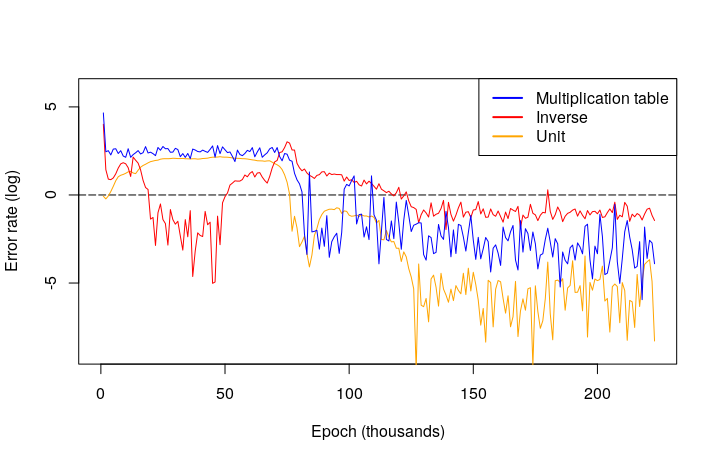
\includegraphics[width=\linewidth]{../img/z20_90percent.png}
\end{figure}

\begin{figure}[h]
\centering
\caption{Values for the half in different $\mathbb{Z}_{20}$ runs. Once again, the reason for why the red one is so different is unknown. The tendency towards 0.5 instead of 10.5 can be attributed to the fact that the initial parameters have been restricted to avoid overflow errors.}
\label{table:z20_half}
\begin{tabular}{|c|c|c|c|c|}
\hline
0.4999506 & \textcolor{red}{-6.5685954} & \textcolor{blue}{10.500707} & 0.49987993 & 0.5000777\\
\hline
0.49967808 & 0.49978873 & 0.49993014 & 0.50047106 & \textcolor{blue}{10.499506}\\
\hline
\end{tabular}
\end{figure}

\begin{figure}[h]
\centering
\caption{An example of a group generated from the "half" element. We see that there were no problems with addition of the half, except the modulus is not applied correctly.}
\label{graph:z20_half_generator}
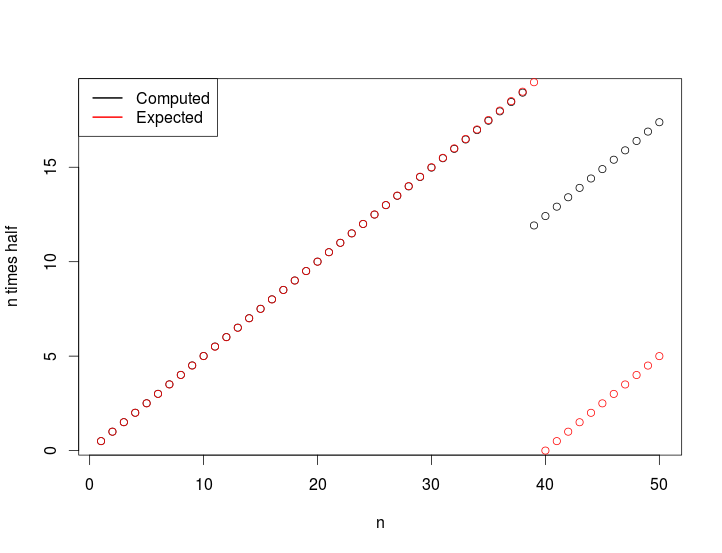
\includegraphics[width=0.8\linewidth]{../img/z20_half_plot.png}
\end{figure}

\subsection{Infinite group $\mathbb{Z}$}
The last cyclic group experiment was with the infinite group $(\mathbb{Z},+)$.

\begin{itemize}
	\item[\textbf{Elements:}] Integers $\dots-2,-1,0,1,2,\dots$
	\item[\textbf{Operations:}] Composition is classic addition, inverse is - and unit is 0.
	\item[\textbf{Grounding:}] As themselves in $\mathbb{R}^1$
	\item[\textbf{Extension:}] Using the equation $h+h=1$. Because of parity, there is no solution in $\mathbb{Z}$.
	\item[\textbf{Notes:}] The extension should be also isomorphic to $\mathbb{Z}$
\end{itemize}

 The training set comprised of integers from an interval $[-10000,10000]$ in order to avoid overflow errors. Because neural network learning is already hard on such a diverse set, we opted to not exclude any data for training.

For the extension $h+h=1$, there is only one intuitive solution: $\frac{1}{2}$. The group generated by this $\frac{1}{2}$ is isomorphic to the original. Unfortunately, we were unable to get to this point. The learned half was 
-1.1713637. When we tried to generate some elements of the extension, we obtained

\begin{tabular}{cccccc}
1&2&3&4&5&6\\
\hline
-1.1713637&1.0000439&2.2069557&2.8777812&3.2506382&3.4578807\\
 \\
7&8&9&10\\
\hline 
3.57307&3.637094&3.6726806&3.6924593
\end{tabular}

Indeed, the learned $h+h=1$, but the composition fails for larger iterations.
\begin{figure}
\caption{$\mathbb{Z}$ as an infinite group. Because of limitations of the software, we only trained on the interval $[-10000,10000]$ (hence the trained group is not really infinite). There was no testing set, but the network seemed to generalize well even outside of the training interval. Examples are computed $11000^{-1}=-11001.614$ or $15000+(-12000)=2999.9941$.}
\centering
\label{graph:z_inf}
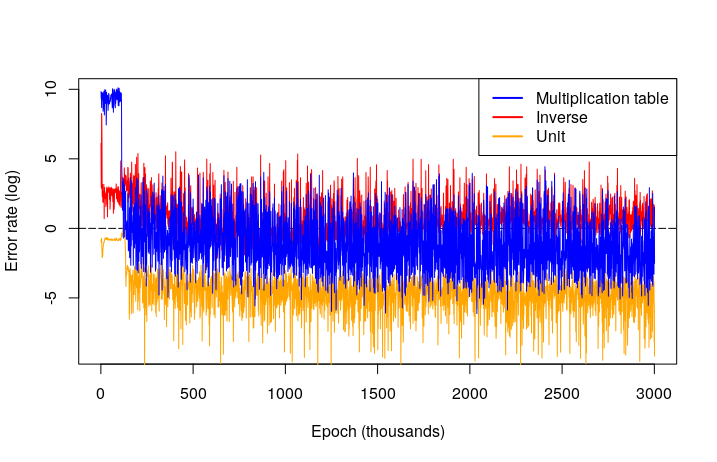
\includegraphics[width=\linewidth]{../img/z_inf.png}
\end{figure}

\section{Symmetric groups}
Symmetric groups, or permutation groups are the most complex finite groups. Indeed, a corollary from Cayley's theorem  is that every finite group is isomorphic to a symmetric group of large enough size (\cite{cayley}). This is why they have been chosen for further experiments.

Every symmetric group is generated by the set of transpositions of two elements. Each element can therefore be written as a sequence of transpositions\footnote{A transposition is the swap of two elements.}. Although this sequence is not unique, all such sequences have the same length. For each permutation $\sigma$ we define $\text{sgn}(\sigma)=(-1)^l$ where $l$ is this number of transpositions. It also holds that $\text{sgn}(\sigma_1\circ\sigma_2)=\text{sgn}(\sigma_1)\text{sgn}(\sigma_2)$. Therefore $\text{sgn}(\sigma\circ\sigma)=1$. (proofs in \cite{Lingebra})

For this reason the equation that we sought to find the extension for is $h\circ h=(0,1)$ where $(0,1)$ denotes the transposition of elements $0$ and $1$. $\text{sgn}((0,1))=-1$, therefore we know that $h$ can not be in the original group. 

Since the symmetric groups are not commutative, we expect this extension to be infinite (see the note after Theorem\autoref{theorem:abelian uniqueness}).

\subsection{$S_4$ with a basic grounding}
$S_4$ is the group of permutations of 4 elements. 

\begin{itemize}
	\item[\textbf{Elements:}] Permutations of a set of 4 elements. We will denote the set as $\{0,1,2,3\}$ and each permutation as $(a,b,c,d)$, where $\{a,b,c,d\}=\{0,1,2,3\}$
	\item[\textbf{Operations:}] Composition is the chaining of permutations, the inverse  of $a$ can be for example obtained by writing $a$ as a sequence of transpositions and reversing their order. The unit is the identity permutation $(0,1,2,3)$.
	\item[\textbf{Grounding:}] Basic grounding means that we encode a permutation $(a,b,c,d)$ as $(a,b,c,d)^\top \in \mathbb{R}^4$.
	\item[\textbf{Extension:}] Using the equation $h\circ h=(1,0,2,3)$. As mentioned above, this has no solution in $S_4$.
	\item[\textbf{Notes:}] 
	\begin{enumerate}
		\item We expect this extension to be infinite, therefore we will not test it all. However, $h^4$ should be $(0,1,2,3)$, which we can use to verify the correctness of the extension.
	
	\item The grounding used here is very short and simple. However, it has a disadvantage in the fact that the mean squared error loss function is biased. We can see this on an example where $[0,1,2,3]$ is one transposition away from both $[1,0,2,3]$ and $[3,1,2,0]$, however in the latter case the mean squared error is considerably higher.
	\end{enumerate}
\end{itemize}


For the training we once again use only 90\% of the data. During the training we expectedly observe significantly higher training times, as exemplified in \Autoref{graph:s4_basic}. This is also compounded by having slightly more elements (24). We are also unable to achieve the same precision. Learning of the unit was again very precise, see table \ref{table:s4_unit_basic}.

When it comes to learning of $h$, we see even more problems than in the case of cyclic groups. Some half elements are seen in table \ref{table:s4_half_basic}. They are noticeably different from each other, something we did not observe before.

However, as we see in table \ref{table:s4_half_basic_gen}, generating even a small subgroup results in a failure. We expect that $h^4=e$, but unfortunately we were never able to get this equation to hold with $h\circ(h\circ(h\circ h))))$. However, because $(h\circ h)\circ (h\circ h)$ yielded reasonable results, we suspect that is the problem is with associativity.

\begin{figure}
\caption{One run of learning the $S_4$ with the basic grounding. This graph shows error rates on 10\% testing data. We see that the training is expectedly much slower than in the cyclic groups.}
\label{graph:s4_basic}
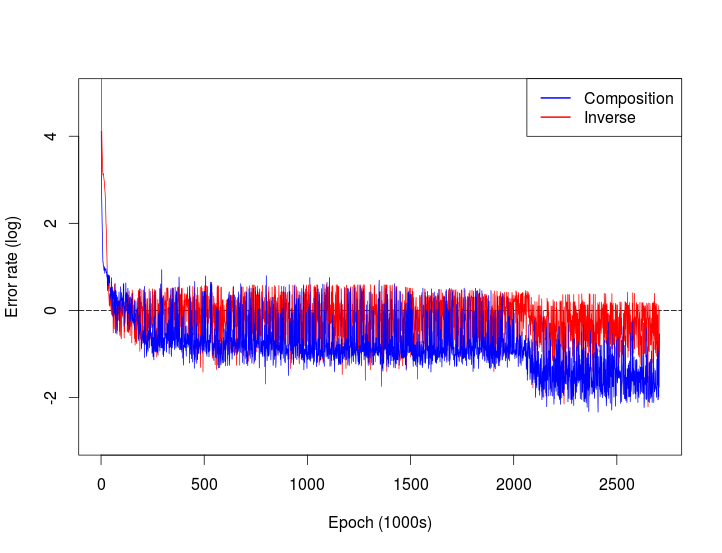
\includegraphics[width=0.9\linewidth]{../img/s4_comp+inv.png}
\end{figure}

\begin{figure}
\center
\caption{Units learned in $S_4$ with basic grounding. The expected output was $[0,1,2,3]$. As we see, they are very precise.}
\label{table:s4_unit_basic}
\begin{tabular}{l|cccc}
1.) &0.03967234 & 1.0745986 & 1.957876 & 2.9761093\\
\hline
2.) &0.00685234 & 1.0557759 & 2.1151063 & 3.2438033\\
\hline
3.) &0.01609807 & 0.9784863 & 2.011951 & 3.0008512\\
\end{tabular}
\end{figure}

\begin{figure}
\center
\caption{$h$-s found in several runs. As expected, they do not look like anything.}
\label{table:s4_half_basic}
\begin{tabular}{l|cccc}
1.)&-0.9288303 & 1.8216157 & 0.17884427 & 2.0224957\\
\hline
2.)&1.2200519 & 0.5469334 & 3.7773933 & -0.22675751\\
 \hline
3.)&2.9790108 & 2.5041845 & 1.9638568 & -1.186425\\
\end{tabular}
\end{figure}

\begin{figure}
\center
\caption{$h$ composed with itself several times. $h^2$ and $h^6$ should both be $[1,0,2,3]$. $h^4$ should be $[0,1,2,3]$.}
\label{table:s4_half_basic_gen}
\begin{tabular}{c|cccc}
$h$   & 2.9790108 & 2.5041845 & 1.9638568 & -1.186425\\
$h^2$ & 1.0137038 & 0.6440371 & 1.960084 & 3.0298772\\
$h^3$ & 1.899735 & 0.6546894 & 2.3109381 & 2.1213117\\
$h^4$ & 1.4959755 & 0.52787334 & 2.564281 & 2.4759564\\
$h^5$ & 1.3819728 & 0.7297171 & 2.8694618 & 2.1578472\\
$h^6$ & 1.1029358 & 0.97653824 & 3.1764572 & 1.9179444\\

\end{tabular}
\end{figure}

\subsection{$S_4$ with matrix grounding}
To fix the problem with the bias of the loss function we change the grounding to the matrix representation.

\begin{itemize}
	\item[\textbf{Elements:}] As above
	\item[\textbf{Operations:}] As above
	\item[\textbf{Grounding:}] A permutation $(a,b,c,d)$ is first encoded as a 4x4 matrix that has ones at the coordinates $(1,a+1),(2,b+1),(3,c+1),(4,d+1)$ and zeros elsewhere. This matrix is then "flattened" into a vector in $\mathbb{R}^{16}$.
	\item[\textbf{Extension:}] As above, $h\circ h=(1,0,2,3)$.
	\item[\textbf{Notes:}] 
	\begin{enumerate}

		\item This grounding erases the loss function bias, because the mean squared difference between any two permutations now only depends on the number of elements switched.
	
		\item Composition of the elements corresponds with matrix multiplication of their groundings, i.e. $\mathcal{G}(p\circ q)=\mathcal{G}(p)\mathcal{G}(q)$.	
	\end{enumerate}	
\end{itemize}

With this grounding, we might encounter a problem with the extension. Assuming the neural network for composition perfectly mimics the matrix multiplication, there is no $h$ in $\mathbb{R}^{4x4}$ that would solve the equation. We can show this using diagonalisation. We can write any (invertible) matrix $A$ as the product $SDS^{-1}$ where $D$ is diagonal and $S$ is orthogonal, where this decomposition is unique (\cite{Lingebra}). From this uniqueness follows that if $B^2=A$ then $B$ is $S\sqrt{D}S^{-1}$ in its diagonalised form, where $\sqrt{D}$ is a diagonal matrix with the elements being the square roots of the elements of $D$. 

We will look at the diagonalisation of the matrix grounding of the element $(1,0,2,3)$.

$$\mathcal{G}(1,0,2,3)=
\left(\begin{matrix}
	0&1&0&0\\
	1&0&0&0\\
	0&0&1&0\\
	0&0&0&1
\end{matrix}\right)
=
\left(\begin{matrix}
	-1&0&0&1\\
	1&0&0&1\\
	0&0&1&0\\
	0&1&0&0
\end{matrix}\right)
\left(\begin{matrix}
	-1&0&0&0\\
	0&1&0&0\\
	0&0&1&0\\
	0&0&0&1
\end{matrix}\right)
\left(\begin{matrix}
	-\frac{1}{2}&\frac{1}{2}&0&0\\
	0&0&0&1\\
	0&0&1&0\\
	\frac{1}{2}&\frac{1}{2}&0&0
\end{matrix}\right)
$$

Unfortunately, $D$ has negative number in it. Therefore $\sqrt{D}$ does not exist in $\mathbb{R}^{4x4}$. Therefore if we are using this grounding we must hope that the optimization process actually avoids the perfect solution for matrix multiplication. This had been fortunately avoided, as seen in the table \ref{table:s4_matrix_half}.

As we can see in \Autoref{graph:s4_matrix}, this representation is still  efficient for composition, but the inverse is clearly wrong. Furthermore, as we see in table \ref{table:s4_matrix_unit}, the unit was usually significantly different from what was expected (an identity matrix). This is a consequence of the networks not being forced to produce $S^m\rightarrow S$ functions, as discussed in \Autoref{section:building_models}.

As a consequence, the inverse is not able to output elements of the grounding. If it did, composition would also output $a^{-1}a$ in grounding, but the learned $e$ is not in it. This is probably the reason for the inverse having such a bad error rate.\\

The learned extension element $h$ is shown in table \ref{table:s4_matrix_half} along with parts of the generated subgroup. Just like with basic grounding, $h\circ h$ shows promise, but $h^4$ breaks down.

\begin{figure}
\center
\caption{$S_4$ with matrix grounding. The testing data percentage is 5\% The composition is very successful, but the inverse is not.}
\label{graph:s4_matrix}
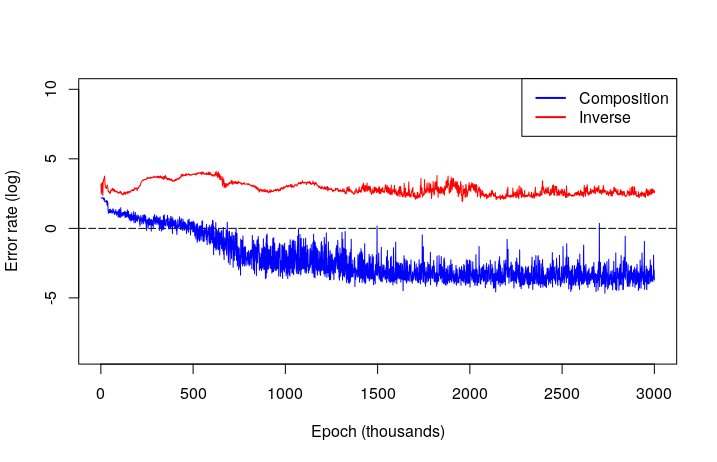
\includegraphics[width=\linewidth]{../img/s4_matrix.png}
\end{figure}

\begin{figure}
\center
\caption{Units found in $S_4$ with matrix representation. An identity matrix was expected. Places where 1 was expected are blue, black ones are for 0.}
\label{table:s4_matrix_unit}
\begin{tabular}{cccc}
\textcolor{blue}{0.9291287} & 0.39432997 & -0.09073094 & -0.00462165\\
-0.49930313 & \textcolor{blue}{2.5813785} & -1.0001388 & -0.51179993\\
0.38528794 & 0.32126167 & \textcolor{blue}{1.4879085} & -0.3122037\\
0.16110185 & -0.10436057 & -0.3780875 & \textcolor{blue}{1.356762}\\
 \\
\hline
\\
 \textcolor{blue}{0.36581007} & 0.11518399 & -0.29025748  & 0.7275856\\
0.38638538 & \textcolor{blue}{0.95944846} & -0.47597495 & -0.14604506\\
0.203323 & -0.15147878 & \textcolor{blue}{0.65808797} & -0.03862157\\
0.4341608 & -0.57306635 & -0.15940993 & \textcolor{blue}{1.5463064}
\end{tabular}
\end{figure}

\begin{figure}
\center
\caption{An extension attempt for $S_4$ with matrix representation. The blue numbers are expected to be $1$ and black ones $0$. As we see, $h^2$ is pretty much exactly what we wanted, but $h^4$ breaks down.}
\label{table:s4_matrix_half}
\begin{tabular}{lcccc}

$h$&-0.44275028 & 0.45813385 & 0.84849375 & -0.4929848\\
 &0.29338264 & 0.25557452 & 0.701611 & -0.33617198\\
 &0.5497755 & 0.75910103 & -0.16280994 & -0.17575327\\
 &0.20515643 & 0.25966993 & 0.10358979 & 1.0272595\\
 
 \hline
 
$h\circ h$&0.0016880417 & \textcolor{blue}{0.99703968} & -0.0002135747 & -0.0009868203\\
 &\textcolor{blue}{0.99901026} & -0.0018832732 & -0.0010174632 & 0.0011361403\\
 &-0.0027710588 & -0.0013556076 & \textcolor{blue}{1.0073379} & -0.001112761\\
 &-0.0005431428 & 0.0049326816 & -0.0010595275 & \textcolor{blue}{1.00323}\\
 
 \hline
 
 $h^4$&\textcolor{blue}{0.72058374} & 0.17218184	& 0.04241377 & 0.04261543\\
&0.4558762 & \textcolor{blue}{-0.00405501}	& 0.55539876 & 0.00293861\\
&-0.02832983 & 0.10163078 & \textcolor{blue}{0.4973646} & 0.4502491\\
&-0.02180864 & 0.6911213	& -0.02542126 &	\textcolor{blue}{0.4643306}

\end{tabular}

\end{figure}